\section{Model, Training, and Validation}
\label{sec:model}
\subsection{Why a small regularized linear model?}
The specification asks whether a compact summary of recent price behavior contains a useful conditional-mean signal. A linear model estimates the joint contribution of the five inputs without expanding the search into transformations and interactions. This is a substantive restriction: the expected return is represented as an additive function of recent returns, price location, and volatility. The volatility coefficient changes the expected-return forecast; it does not mechanically scale the position by inverse volatility.

The main estimation concern is the combination of noisy daily outcomes and overlapping predictors. Five- and twenty-session returns share observations, and the moving-average gap also summarizes the recent price path. Ordinary least squares can allocate large, offsetting coefficients to similar inputs. Ridge penalizes the squared size of that coefficient vector, favoring a more stable joint forecast. Here there are five inputs and 1,260 training observations, so shrinkage addresses estimation variability rather than a shortage of observations relative to predictors.

Retaining all five inputs also matches the research premise. Each represents a related but distinct summary of recent behavior, and the design does not assume that only one is relevant. Ridge therefore provides a natural alternative to a sparsity penalty such as LASSO, which can remove predictors entirely. A larger nonlinear model would require additional choices about interactions, capacity, and tuning. The implemented experiment instead concentrates its model search on one transparent source of flexibility, the shrinkage strength. These are design reasons for the chosen estimator; the empirical comparison is against the recorded forecast and trading benchmarks.

\subsection{Ridge estimation on past-only standardized inputs}
At each refit date $d$, means $\mu_d$ and population standard deviations $s_d$ are estimated on $\mathcal T_d$. For each feature coordinate, the standardized value is
\begin{equation}
z_{t,d}=(x_t-\mu_d)\oslash s_d,
\label{eq:standardize}
\end{equation}
where $\oslash$ denotes coordinatewise division. The same transformation is used for subsequent predictions until the next refit. The model minimizes
\begin{equation}
(\widehat a_d,\widehat\beta_d)
=\arg\min_{a,\beta}\left\{
\sum_{t\in\mathcal T_d}(y_t-a-z_{t,d}^{\mathsf T}\beta)^2
+\alpha\|\beta\|_2^2\right\}.
\label{eq:ridge}
\end{equation}
The intercept is unpenalized. The implemented loss is a sum of squares, so $\alpha$ has the scikit-learn Ridge convention \citep{sklearnridge}.

The penalty shrinks coefficients that would otherwise be sensitive to overlapping return predictors. For centered training data with singular-value decomposition $Z=USV^{\mathsf T}$, the solution can be written as
\begin{equation}
\widehat\beta_d=V\operatorname{diag}\!\left(\frac{s_j}{s_j^2+\alpha}\right)U^{\mathsf T}y_c.
\label{eq:svd}
\end{equation}
This replaces the least-squares amplification $1/s_j$ by $s_j/(s_j^2+\alpha)$, reducing sensitivity in directions with small singular values. Standardization makes the penalty comparable across features measured on different scales. The implementation uses a \code{StandardScaler}/\code{Ridge} pipeline with the SVD solver. It does not use stochastic gradient training.

The unpenalized intercept gives the historical-mean benchmark a direct interpretation. Since the standardized training columns have zero mean, minimizing Eq.~\eqref{eq:ridge} over the intercept yields
\begin{equation}
\widehat a_d=\overline y_d,\qquad
\widehat y_t=\overline y_{d(t)}+z_{t,d(t)}^{\mathsf T}\widehat\beta_{d(t)}.
\label{eq:meanadjustment}
\end{equation}
Ridge thus adds a conditional adjustment to the same past-only mean used by the prediction reference. Increasing $\alpha$ shrinks the adjustment toward zero; in the limit the forecast approaches that reference. This separates an estimated average equity return from the incremental information attributed to the five features.

The model is fitted on the first evaluation signal and the first decision session of each new calendar month. Each fit uses the latest 1,260 mature labels, with a minimum requirement of 1,000. Between fits, the coefficients and scaler remain fixed, while new daily features change the forecasts. If $d(t)$ denotes the latest refit date, then
\begin{equation}
\widehat y_t=\widehat a_{d(t)}+z_{t,d(t)}^{\mathsf T}\widehat\beta_{d(t)}.
\label{eq:forecast}
\end{equation}

The five-year window balances a substantial estimation sample against the use of a full expanding history whose oldest observations never leave the fit. Monthly updates allow the estimated relationship to change on a regular schedule while avoiding daily coefficient re-estimation. Daily decisions still respond to new features between refits. The window and update frequency are fixed parts of the specification, so the validation search compares four penalties under the same adaptation rule rather than jointly searching over many training designs.

\subsection{Chronological split and forward validation}
The initial development history is 2010--2018. Holding intervals within 2019--2021 form the validation period, and intervals within 2022--2025 form the final evaluation. Period membership is defined by both entry and exit dates. This gives the test entry on 3 January 2022 and liquidation at the 31 December 2025 open.

Forward validation reproduces the intended use of the model: fit with outcomes already realized, issue a forecast, and move to the next decision. Randomly shuffled folds would allow later observations to inform forecasts for earlier dates and would break that deployment sequence. The label-exit filter in Eq.~\eqref{eq:train} handles the additional execution delay explicitly. Adjacent holding intervals share an opening-price boundary but do not share the same holding return; eligibility is determined by when the entire label is observed, rather than by an arbitrary gap between rows.

\begin{figure}[!htbp]
\centering
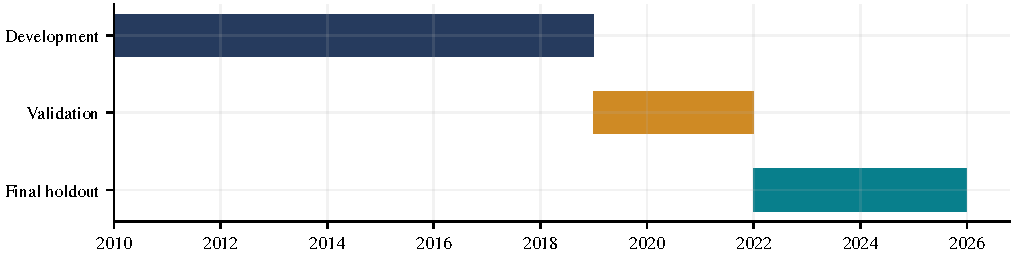
\includegraphics[width=.96\textwidth]{figures/timeline.pdf}
\caption{Chronology of the research design. All fits use the latest 1,260 fully realized labels. The penalty is selected using validation performance and then held fixed during final evaluation.}
\label{fig:timeline}
\end{figure}

Four penalty values, $\alpha\in\{0.1,1,10,100\}$, are walked forward through validation. Each candidate has its own monthly past-only fits and daily position path. The selection criterion is net validation Sharpe at a single-side cost of 5 basis points. Ties within $10^{-12}$ are resolved in favor of the larger penalty. Table~\ref{tab:validation} reports every candidate.

\begin{table}[!htbp]
\centering\small
\caption{Forward validation, 2019--2021: the complete four-candidate search.}
\label{tab:validation}
\begin{tabular}{@{}rrrrrr@{}}
\toprule
$\alpha$ & CAGR (\%) & Net Sharpe & Exposure (\%) & Turnover & $R^2_{\mathrm{OOS}}$ \\
\midrule
0.1 & 22.33 & 1.2060 & 76.72 & 136 & -0.01442 \\
1 & 22.33 & 1.2060 & 76.72 & 136 & -0.01434 \\
10 & 19.15 & 1.0767 & 77.38 & 134 & -0.01364 \\
100 & 18.64 & 1.0310 & 85.71 & 116 & -0.01089 \\
\bottomrule
\end{tabular}

\tabnote{Each candidate is evaluated on 756 holding intervals at 5 bps. CAGR and exposure are percentages; turnover counts charged one-way trade units. $R^2_{\mathrm{OOS}}$ uses the past-only historical-mean reference and is reported as a diagnostic.}
\end{table}

Penalties 0.1 and 1 produce identical validation position signs and hence identical trading results. Their continuous forecasts differ, but the tie rule selects $\alpha=1$. Larger penalties have lower validation Sharpe. Forecast MSE is calculated as a diagnostic; it is not an additional selection objective. This distinction matches the research question: estimation minimizes squared prediction error, while validation selects the regularization strength for the trading application.

The grid illustrates why those objectives differ. At $\alpha=100$, validation $R^2_{\mathrm{OOS}}$ improves from approximately $-0.01434$ to $-0.01089$, yet net Sharpe falls from 1.2060 to 1.0310. The sign rule depends on which scores cross zero, not on their squared errors alone. Exposure rises from 76.72\% to 85.71\%, while turnover falls from 136 to 116 units. Stronger shrinkage therefore changes both the held-return subset and its implementation costs. The stated Sharpe rule resolves that trade-off without selecting a different criterion after observing the final period.

\subsection{Final rolling evaluation and overfitting control}
The selected penalty is used throughout final evaluation. Earlier test outcomes enter later training windows once their exit dates have passed. The model therefore adapts through a fixed rolling rule rather than remaining fitted to a single pre-2022 sample. The final path contains 49 fits: an initial fit at the 31 December 2021 close, followed by the first decision session in each month of 2022--2025. Every test fit contains 1,260 eligible observations.

The search is restricted to four penalties for one asset, one feature set, one training-window length, and one monthly update schedule. The forecast threshold and moving-average benchmark are fixed. These choices control the number of alternatives considered, while Ridge controls coefficient size within each alternative. Training-only scaling and the label-maturity filter separately control information leakage.

The procedure is implemented in four stages:
\begin{enumerate}
\item Construct trailing features and the opening-to-opening target; retain fully defined observations.
\item Walk each penalty through validation, using Eq.~\eqref{eq:train} at every refit, and account for the resulting trades at the declared cost.
\item Select $\alpha$ using the stated Sharpe and tie rules; record the protocol, input, and validation-table fingerprints.
\item Generate the selected model's test forecasts and positions, then save daily accounting paths, monthly fit audits, and evaluation tables.
\end{enumerate}
The exported audit records make the correspondence between training and testing explicit. Unit checks also change future prices and verify that earlier features, fits, scalers, and forecasts remain unchanged. Source functions and reproduction commands are listed in Appendix~\ref{app:reproduction}.
